\documentclass[12pt]{article}
\usepackage[utf8]{inputenc}
\usepackage{amsmath}
\usepackage{amssymb}
\usepackage{amsthm}
\usepackage{fullpage}
\usepackage{graphicx}
\usepackage{hyperref}
\usepackage{enumitem}
\usepackage{algorithm2e}
\usepackage{float}
%% Sets page size and margins
\usepackage[a4paper,top=2.5cm,bottom=2.5cm,left=2cm,right=2cm]{geometry}


%% Title
\title{
		\vspace{-0.7in}
		\usefont{OT1}{bch}{b}{n}
		\begin{minipage}{3cm}
        \vspace{-0.5in}
    	\begin{center}
    		
\includegraphics[height=3.2cm]{../logo_unam.png}
    	\end{center}
    \end{minipage}\hfill
    \begin{minipage}{10.7cm}

    	\begin{center}
\normalfont \normalsize \textsc{UNIVERSIDAD NACIONAL AUTÓNOMA DE MÉXICO \\ FACULTAD DE CIENCIAS \\ Análisis de Algoritmos } \\
		\huge Tarea 3
    	\end{center}

    \end{minipage}\hfill
    \begin{minipage}{3.2cm}
    \vspace{-0.5in}
    	\begin{center}
    		
\includegraphics[height=3.2cm]{../logo_fc.png}
    	\end{center}
    \end{minipage}

\author{Escobar Gonzalez Isaac Giovani \hspace{1cm} 321336400\\
        Garduño Escobar Kevin Jonathan \hspace{0.5cm} 321070629\\
        Zaldivar Alanis Rodrigo \hspace{2.75cm} 424029605 }
\date{}
}

\begin{document}

\maketitle

\section*{Ejercicio 1}
Considera el siguiente algoritmo:\\
\RestyleAlgo{ruled}
\LinesNumbered
\renewcommand{\algorithmcfname}{Algoritmo}
\begin{algorithm}[H]
    Algoritmo: ordenamientoMisterioso( A, n )\\
    \If{$n == 2 \; \& \; A[0] > A[1]$}{
        intercambiar $A[0] \longleftrightarrow A[1]$\;
    }
    \ElseIf{ $n > 2$ } {
        $m = \lceil 2n/3\rceil$\;
        $ordenamientoMisterioso(A[0 .. m-1])$ \;
        $ordenamientoMisterioso(A[n-m .. n-1])$ \;
        $ordenamientoMisterioso(A[0 .. m-1])$ \;
    }
\end{algorithm}
\begin{itemize}
    \item[1.A] Prueba que el algoritmo es correcto (ordena correctamente la salida)
    \item[1.B] ¿El algoritmo es estable?
    \item[1.C] ¿El algoritmo utiliza es $in$ - place (utiliza memoria constante) ?
    \item[1.D] Realiza el análisis de complejidad de tiempo. Plantea y resuelve la ecuación de recurrencia. Concluye mencionando la complejidad asintótica.
    \item[1.E] Si cambiamos $m = \lceil 2n/3 \rceil$ por $m = \lfloor 2n/3 \rfloor$, ¿el algoritmo aún es correcto? Justifica
\end{itemize}
\section*{Ejercicio 2}
Se tienen dos arreglos $A, B$ de longitudes $m, n$ respectivamente. Diseña un algoritmo de tiempo $O(m + n)$ que construya un arreglo $C$ con los elementos en común entre $A$ y $B$, sin elementos repetidos.
\begin{itemize}
    \item[2.A] Da el pseudocódigo
    \item[2.B] Realiza el análisis de correctitud
    \item[2.C] Realiza el análisis de complejidad en tiempo
    \item[2.D] Realiza el análisis de complejidad en espacio
    \item[2.E] Menciona algunos casos interesantes (incluyendo un mejor y peor caso). Ilustra con ejemplos concretos.
\end{itemize}
\section*{Ejercicio 3}
Supón que tenemos un algoritmo en el cual vamos a utilizar pilas (Stacks) pero no conocemos el máximo de elementos a almacenar. Usando arreglos dinámicos, propón una estrategia para trabajar con pilas.
\begin{itemize}
    \item[3.A] Realiza el análisis de la complejidad de tiempo y espacio para las operaciones de la pila (push, pop)
    \item[3.B] Supón que queremos ahorrar el espacio que no se está utilizando, por lo cual se propone reducir el tamaño máximo de la pila a la mitad, cada que la pila reduzca su tamaño a la mitad de elementos. ¿Cómo se modifica el análisis de complejidad del inciso anterior?
    \item[3.C] ¿Cómo se modificaría las respuestas a los incisos anteriores si en vez de una pila consideramos una cola?
\end{itemize}
\section*{Ejercicio 4}
Investiga en qué consiste el método (o teorema) maestro.\\
Ilustra su aplicación con algunos ejemplos.\\
Nota: NO es necesario presentar la demostración del teorema en esta tarea, pero sí es deseable que la revisen y comenten de manera general.
\section*{Ejercicio 5}
Para este problema, considera que un subárbol de un árbol binario es cualquier subgráfo conexo. Un árbol binario es completo sí todos los nodos internos tienen dos hijos y cada hoja tiene exactamente la misma profundidad.\\
Describe un algoritmo para calcular el subárbol completo más grande (mayor número de nodos). El algoritmo debería devolver el nodo (o referencia) al subárbol y la altura correspondiente.
\begin{itemize}
    \item[5.A] Da el pseudocódigo
    \item[5.B] Realiza el análisis de complejidad en tiempo
    \item[5.C] Realiza el análisis de correctitud
\end{itemize}
\begin{figure}
    \centering
    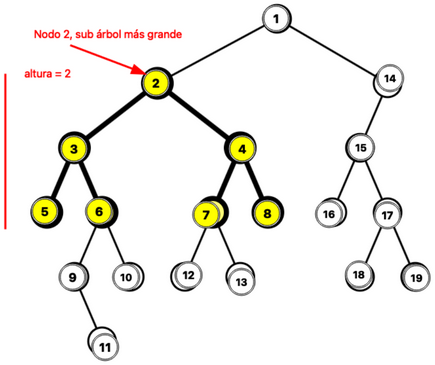
\includegraphics[width=0.7\textwidth]{subárbol.png}
    \caption{Ejemplo de un subárbol binario completo.\\
    En amarillo se indican los nodos correspondientes al subárbol completo más grande.}
\end{figure}

\end{document}
